\documentclass{tudelft-report}

%% Set up the bibliography
\usepackage{biblatex}
\addbibresource{report.bib}

%% Additional packages and commands
\usepackage{parskip}
\setlist{itemsep=-2pt} % Reducing white space in lists slightly
\renewcommand{\deg}{\si{\degree}\xspace} % Use \deg easily, everywhere
\usepackage{tcolorbox}

%% ----------------------------------------------------------------------
%%    Begin of document + Frontmatter (Roman page numbering)
%% ----------------------------------------------------------------------

\begin{document}

\frontmatter

%% Define the main parameters
\title{\textbf{Laboratorio} \\ Extracción de características y bolsa de palabras visuales}
\author{Ingeniería Matemática}

\subject{Visión por Ordenador I} % Cover only
\affiliation{Universidad Pontificia Comillas, ICAI} % Cover only
\coverimage{figures/cover.jpg} % Aspect ratio of 2:3 (portrait) recommended
\definecolor{title}{HTML}{ffffff} % Color for cover title

\makecover

\begin{titlepage}

\begin{center}

\bigskip
\bigskip

%% Print the name of the author
{\makeatletter
\begin{tabular}{c}
    3º \@author \\\midrule
    Curso 2025/26
\end{tabular}
\makeatother}

\bigskip
\bigskip

%% Print the title
{\makeatletter
\largetitlestyle\fontsize{45}{45}\selectfont\@title
\makeatother}

%% Print the subtitle
{\makeatletter
\ifdefvoid{\@subtitle}{}{\bigskip\titlestyle\fontsize{20}{20}\selectfont\@subtitle}
\makeatother}

%% Print table with names; easily add columns if necessary or remove the table completely
% \setlength\extrarowheight{2pt}
% \begin{tabular}{c}
%     3º  \\\midrule
%     Curso 2024/25 \\
% \end{tabular}

\vfill

%% Print some more information at the bottom
\begin{tabular}{ll}
    \textbf{Profesor}: & \textbf{Email} \\
    Erik Velasco & evelasco@icai.comillas.edu \\
    Lionel Güitta & lglopez@icai.comillas.edu \\
    Daniel Pinilla & dpinilla@icai.comillas.edu \\
    Luis Arias & learias@icai.comillas.edu \\
    José María Bengochea & jmbengochea@icai.comillas.edu \\ 
    Mario Triviño & mtrivino@comillas.edu \\
\end{tabular}

\bigskip
\bigskip

%% Add a source and description for the cover and optional attribution for the template
\begin{tabular}{p{15mm}p{10cm}}
    Cover: & Erosion, tectonic uplift, and a human-built dam have all helped shape the Upper Lake Powell area in Utah. Image Credit: NASA \\
    
    % Feel free to remove the following attribution, it is not required - still appreciated :-)
    % Style: & TU Delft Report Style, with modifications by Daan Zwaneveld
\end{tabular}
\vspace{10mm}

\end{center}

%% Insert the Comillas logo at the bottom of the page
\begin{tikzpicture}[remember picture, overlay]
    \node[above=10mm] at (current page.south) {%
        
\includegraphics[scale=0.15]{figures/logo-color}
    };
\end{tikzpicture}

\end{titlepage}

%\chapter*{Preface}
\addcontentsline{toc}{chapter}{Preface}

\emph{A preface...}

\begin{flushright}
{\makeatletter\itshape
    \@author \\
    Delft, \monthname{} \the\year{}
\makeatother}
\end{flushright}

%\chapter*{Summary}
\addcontentsline{toc}{chapter}{Summary}

\emph{A summary...}


\tableofcontents
%\listoffigures
%\listoftables

%\chapter*{Nomenclature}
\addcontentsline{toc}{chapter}{Nomenclature}

\emph{If a nomenclature is required, a simple template can be found below for convenience. Feel free to use, adapt or completely remove.}

\section*{Abbreviations}

\begin{longtable}{p{2.5cm}p{8cm}}
    \toprule
    Abbreviation & Definition \\
    \midrule\endhead % Add abbreviations alphabetically here:
    ISA & International Standard Atmosphere \\
    ... \\
    \bottomrule
\end{longtable}

\section*{Symbols}

\begin{longtable}{p{2.5cm}p{8cm}p{2.5cm}}
    \toprule
    Symbol & Definition & Unit \\
    \midrule\endhead % Add Latin symbols alphabetically here:
    $V$ & Velocity & [m/s] \\
    ... \\
    \midrule % Add Greek symbols alphabetically here:
    $\rho$ & Density & [kg/m$^3$] \\
    ... \\
    \bottomrule
\end{longtable}


%% ----------------------------------------------------------------------
%%    Mainmatter (Arabic page numbering)
%% ----------------------------------------------------------------------

\mainmatter

\chapter{Sesión 4: Detección de Movimiento y Seguimiento de Objetos}
\label{chapter:introduction_ses_4}

\section{Materiales}

En esta práctica se trabajará con los siguientes recursos (puede encontrarlos en la sección de Moodle \textit{Laboratorio/Sesión 4}):

\begin{itemize}
    \item \textbf{\texttt{lab4.ipynb}}: notebook con el código que deberá desarrollar.
    \item \textbf{data}: carpeta con vídeos para trabajar durante la práctica.
\end{itemize}

\section{Apartados de la práctica}

La Sesión 4 del laboratorio está dividida en los siguientes apartados:

\begin{itemize}
    \item Librerías: Importación de las librerías que se utilizan en la sesión. Se recomienda realizar la importación en una celda inicial para mantener la organización del Notebook.
    \item Apartado A: Sustracción de fondo.
    \item Apartado B: Flujo Óptico.
    \item Apartado D: Filtro de Kalman para Seguimiento de Objetos.
    \item Apartado D: Ejercicio Adicional.
\end{itemize}

\section{Observaciones}

Aunque el guion de la práctica y los comentarios en Markdown del Notebook estén escritos en español, observe que todo aquello que aparece en las celdas de código está escrito en inglés. Es una buena práctica que todo su código esté escrito en inglés.

Aquellas partes del código que deberá completar están marcadas con la etiqueta \textbf{\texttt{TODO}}.

Es muy importante que trabaje consultando la documentación de OpenCV\footnote{\href{https://docs.opencv.org/4.x/index.html}{Documentación de OpenCV}: \url{https://docs.opencv.org/4.x/index.html}} para familiarizarse de cara al examen. Tenga en cuenta que en los exámenes no podrá utilizar herramientas de ayuda como Copilot.

\section{Qué va a aprender}

Al finalizar esta práctica, aprenderá a implementar algoritmos de detección de movimiento mediante sustracción de fondo y flujo óptico, y explorará el filtro de Kalman para el seguimiento de objetos.

\section{Evaluación}

La nota que obtenga en esta sesión de laboratorio será la misma que obtenga su pareja. Los apartados de la práctica serán evaluados como refleja la Tabla \ref{table:evaluacion}.

\begin{table}[h!]
    \centering
    \begin{tabular}{|c|c|c|}
    \hline
    \textbf{Tarea} & \textbf{Valor} & \textbf{Resultado} \\
    \hline
    Pregunta A.1 & 1.5 & \\
    \hline
    Pregunta A.2 & 2.0 & \\
    \hline
    Pregunta B.1 & 1.5 & \\
    \hline
    Pregunta B.2 & 2.0 & \\
    \hline
    Pregunta C.1 & 1.5 & \\
    \hline
    Pregunta C.2 & 1.5 & \\
    \hline
    Pregunta D.1 & 1.0 & \\
    \hline
    Pregunta D.2 & 1.0 & \\
    \hline
    \textbf{Total} & \textbf{12.0} & \\
    \hline
    \end{tabular}
    \caption{Valoración de los apartados de la práctica.}
    \label{table:evaluacion}
\end{table}

\chapter{Apartado A: \textbf{Detección de esquinas}}
\label{chapter:tarea_a}


\section*{Tarea A.1: Creación de carpeta de resultados}
\phantomsection
\addcontentsline{toc}{section}{Tarea A.1: Creación de carpeta de resultados}

Cree una nueva capeta llamada \texttt{partA}, dentro de la carpeta \texttt{data}, con el objetivo de presentar en ella los resultados de esta parte de la práctica.

\section*{Tarea A.2: Carga de imágenes}
\addcontentsline{toc}{section}{Tarea A.2: Carga de imágenes}

Defina y ejecute los dos métodos propuestos para cargar imágenes \texttt{imageio\_load\_images()} y \texttt{opencv\_load\_images()}. Observe lo que ocurre al guardar ambas imágenes usando la misma función \texttt{cv2.imwrite()}.

\section*{Tarea A.3: Definición del método  Harris para detección de esquinas}
\addcontentsline{toc}{section}{Tarea A.3: Definición del método  Harris para detección de esquinas}
Defina la función \texttt{harris\_corner\_detector()}, que servirá para detectar las esquinas de las imágenes de trabajo. Siga los siguientes pasos:

\begin{itemize}
    \item Convertir la imagen de entrada a escala de grises usando \texttt{cv2.cvtColor()}.
    \item Transformar la imagen en escala de grises al tipo \texttt{float32} con \texttt{np.float32}.
    \item Aplicar el método \texttt{cv2.cornerHarris()} \footnote{ \href{https://docs.opencv.org/3.4/dd/d1a/group\_\_imgproc\_\_feature.html\#gac1fc3598018010880e370e2f709b4345}{Documentación del método Harris en OpenCV:} \\{https://docs.opencv.org/3.4/dd/d1a/group\_\_imgproc\_\_feature.html\#gac1fc3598018010880e370e2f709b4345}}.
    \item Dilatar la imagen resultante con \texttt{cv2.dilate} para mejorar la visibilidad de las esquinas detectadas.
    \item Establecer un umbral para resaltar las esquinas detectadas.
\end{itemize}

\section*{Tarea A.4: Aplicación de Harris}
\addcontentsline{toc}{section}{Tarea A.4: Aplicación de Harris}
Aplique la función \texttt{harris\_corner\_detector()} sobre las imágenes de trabajo. Asegúrese de que las imágenes quedan guardadas como se especifica en los comentarios. La Figura \ref{fig:ejemplo_harris} muestra un ejemplo con el resultado que debería obtener al aplicar el método Harris.

\begin{figure}[H]
    \centering
    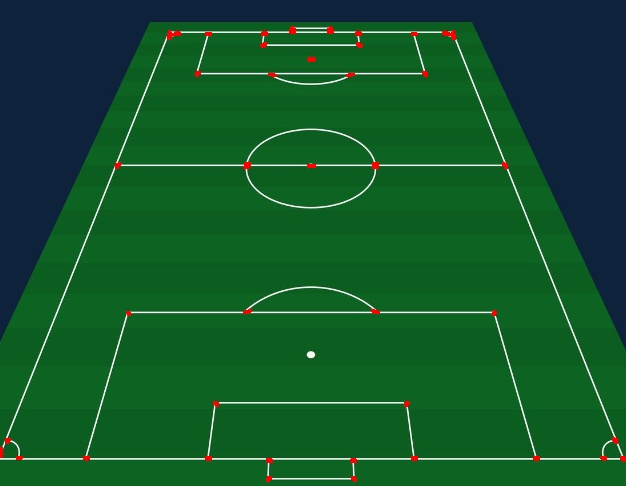
\includegraphics[width=0.3\textwidth]{Lab_3/template/figures/Harris_football.jpg}
    \caption{Ejemplo de detección de esquinas con el método Harris.}
    \label{fig:ejemplo_harris}
\end{figure}


\section*{Tarea A.5: Definición del método  Shi-Tomasi para detección de esquinas}
\addcontentsline{toc}{section}{Tarea A.5: Definición del método  Shi-Tomasi para detección de esquinas}
Defina la función \texttt{shi\_tomasi\_corner\_detection()}, que servirá para la detección de esquinas sobre las imágenes de trabajo. Siga los siguientes pasos:

\begin{itemize}
    \item Convertir la imagen de entrada a escala de grises utilizando \texttt{cv2.cvtColor()}.
    \item Aplicar el método \texttt{cv2.goodFeaturesToTrack()} \footnote{ \href{https://docs.opencv.org/3.4/dd/d1a/group\_\_imgproc\_\_feature.html\#ga1d6bb77486c8f92d79c8793ad995d541}{Documentación del método \texttt{goodFeaturesToTrack()} en OpenCV:} \\{https://docs.opencv.org/3.4/dd/d1a/group\_\_imgproc\_\_feature.html\#ga1d6bb77486c8f92d79c8793ad995d541}}.
    \item Convertir las coordenadas de las esquinas detectadas a enteros utilizando \texttt{np.intp}.
    \item Para cada esquina detectada, extraer las coordenadas \texttt{x} e \texttt{y} y dibujar un círculo en la imagen usando \texttt{cv2.circle()}.
\end{itemize}


\section*{Tarea A.6: Aplicación de Shi-Tomasi}
\addcontentsline{toc}{section}{Tarea A.6: Aplicación de Shi-Tomasi}
Aplique la función \texttt{shi\_tomasi\_corner\_detection()} sobre las imágenes de trabajo. Asegúrese de que las imágenes quedan guardadas como se especifica en los comentarios.

\section*{Preguntas}
\addcontentsline{toc}{section}{Preguntas}

\vspace{5mm}
\begin{tcolorbox}[colback=gray!10, colframe=gray!30, coltitle=black, title=Pregunta A.1, halign=left]
Realice la detección de esquinas en las otras dos imágenes de la carpeta \texttt{data/source} (cuyos nombres de guardado han de ser \textit{sudoku} y \textit{tennis}) con el método de Harris.
\end{tcolorbox}

\vspace{5mm}
\begin{tcolorbox}[colback=gray!10, colframe=gray!30, coltitle=black, title=Pregunta A.2, halign=left]
Realice la detección de esquinas en las otras dos imágenes de la carpeta \texttt{data/source} (cuyos nombres de guardado han de ser \textit{sudoku} y \textit{tennis}) con el método de Shi-Tomasi.
\end{tcolorbox}
\chapter{Apartado B: \textbf{Detección de líneas rectas}}
\label{chapter:tarea_b}

\section*{Tarea B.1: Aplicación de Canny}
\phantomsection
\addcontentsline{toc}{section}{Tarea B.1: Aplicación de Canny}

Para obtener los bordes de las imágenes, aplique el método \texttt{cv2.Canny()} \footnote{ \href{https://docs.opencv.org/3.4/dd/d1a/group\_\_imgproc\_\_feature.html\#ga04723e007ed888ddf11d9ba04e2232de}{Documentación del método \texttt{cv2.Canny()} en OpenCV:} \\{https://docs.opencv.org/3.4/dd/d1a/group\_\_imgproc\_\_feature.html\#ga04723e007ed888ddf11d9ba04e2232de}} de OpenCV a las imágenes de trabajo ajustando los hiperparámetros.

Recuerde que para aplicar Canny, primero deberá pasar su imagen a escala de grises con el método \texttt{cvtColor()}. Por otro lado, observe que el método Canny devuelve una imagen binaria (blanco y negro) con los bordes detectados.


\section*{Tarea B.2: Visualización de líneas}
\phantomsection
\addcontentsline{toc}{section}{Tarea B.2: Visualización de líneas}

Implemente la función \texttt{draw\_lines()} para pintar las líneas detectadas sobre las imágenes. Para ello, puede utilizar el método \texttt{cv2.line()} \footnote{ \href{https://docs.opencv.org/3.4/d6/d6e/group\_\_imgproc\_\_draw.html\#ga7078a9fae8c7e7d13d24dac2520ae4a2}{Documentación del método \texttt{cv2.line()} en OpenCV:} \\{https://docs.opencv.org/3.4/d6/d6e/group\_\_imgproc\_\_draw.html\#ga7078a9fae8c7e7d13d24dac2520ae4a2}} de OpenCV.


\section*{Tarea B.3: Aplicación de transformada de Hough}
\phantomsection
\addcontentsline{toc}{section}{Tarea B.3: Aplicación de transformada de Hough} 
Aplique el método \texttt{cv2.HoughLinesP()} \footnote{ \href{https://docs.opencv.org/3.4/dd/d1a/group\_\_imgproc\_\_feature.html\#ga8618180a5948286384e3b7ca02f6feeb}{Documentación del método \texttt{cv2.HoughLinesP()} en OpenCV:} \\{https://docs.opencv.org/3.4/dd/d1a/group\_\_imgproc\_\_feature.html\#ga8618180a5948286384e3b7ca02f6feeb}} de OpenCV a las imágenes de trabajo y afine los hiperparámetros para extraer las líneas de interés. La Figura \ref{fig:ejemplo_hough} muestra el resultado esperado al aplicar la transformada de Hough sobre una de las imágenes.

\begin{figure}[H]
    \centering
    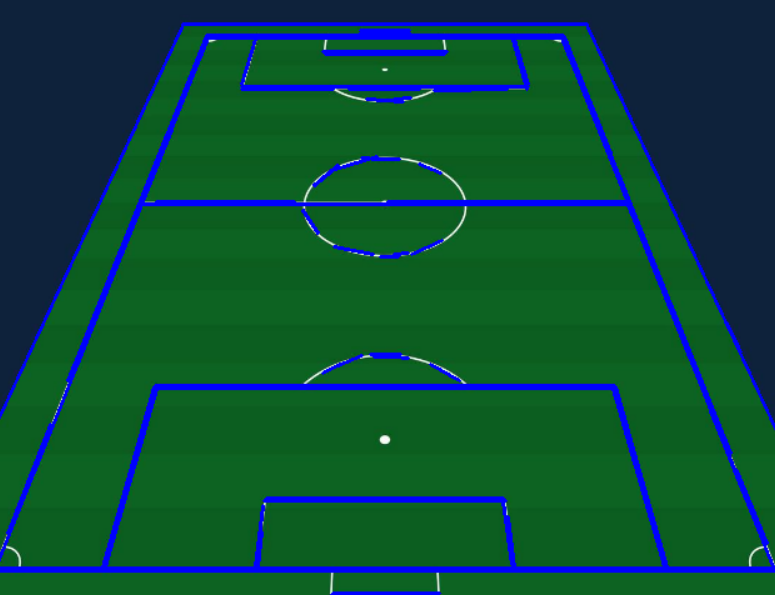
\includegraphics[width=0.3\textwidth]{Lab_3/template/figures/football_lines.png}
    \caption{Ejemplo de detección de líneas con el método Hough.}
    \label{fig:ejemplo_hough}
\end{figure}


\section*{Preguntas}
\addcontentsline{toc}{section}{Preguntas}

\vspace{5mm}
\begin{tcolorbox}[colback=gray!10, colframe=gray!30, coltitle=black, title=Pregunta B.1, halign=left]
Repita el procedimiento para extraer las líneas de las dos imágenes restantes.
\end{tcolorbox}
\chapter{Apartado C: \textbf{Detección de puntos de interés y Bolsa de palabras}}
\label{chapter:tarea_c}

En este apartado deberá extraer los puntos de interés de una de las imágenes de la carpeta \texttt{data}. Una vez hecho, podrá comprobar la correspondencia con esa imagen alterada y la relación entre las mismas (Figura \ref{fig:feat_match}). Tras entender la funcionalidad de este método, pasará a obtener una bolsa de palabras a partir de un \textit{dataset} de entrenamiento y generar predicciones para un \textit{dataset} de evaluación.

\begin{figure}[h]
    \centering
    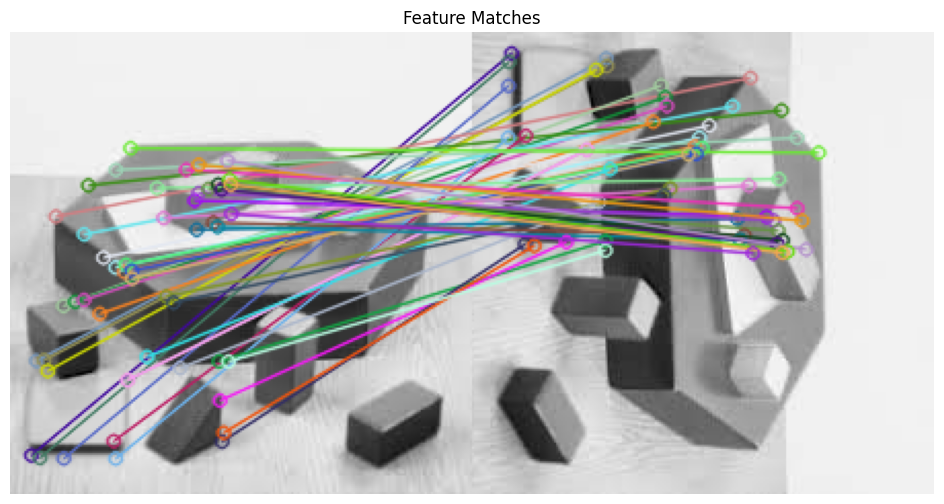
\includegraphics[width=0.6\textwidth]{Lab_3/template/figures/FeatureMatch.png}
    \caption{Correspondencia de características entre una imagen y la misma alterada con OpenCV.}
    \label{fig:feat_match}
\end{figure}

\section*{C.1: Detección de puntos de interés}
\phantomsection
\addcontentsline{toc}{section}{C.1: Detección de puntos de interés}

En esta sección se generarán las funciones necesarias que cubran la detección de puntos de interés y los descriptores para las imágenes empleando la transformación SIFT.
La transformación SIFT consta de cuatro pasos principales:

\begin{enumerate}
    \item Detección de extremos en espacio de escalas.
    \item Localización de keypoints.
    \item Asignación de orientaciones.
    \item Generación de los descriptores de keypoints.
\end{enumerate}

Cada uno se irá desarrollando con las funciones necesarias para completarlos. De esta forma se comenzará generando el espacio de escalas en el que se evaluarán los extremos.

\subsection*{Tarea C.1.1: Filtro gaussiano con OpenCV}
\phantomsection
\addcontentsline{toc}{subsection}{Tarea C.1.1: Filtro gaussiano con OpenCV}

Para generar el espacio de escalas que se desea analizar, se debe aplicar un filtrado gaussiano a la imagen original hasta obtener un número de imágenes gaussianas relevante. Para ello, debe desarrollar la función \texttt{generateGaussianImages()} empleando el método \texttt{cv2.GaussianBlur()} \footnote{ \href{https://docs.opencv.org/3.4/d4/d86/group\_\_imgproc\_\_filter.html\#gaabe8c836e97159a9193fb0b11ac52cf1}{Documentación del método \texttt{cv2.GaussianBlur()} en OpenCV:} \\{https://docs.opencv.org/3.4/d4/d86/group\_\_imgproc\_\_filter.html\#gaabe8c836e97159a9193fb0b11ac52cf1}} de la librería OpenCV.


Como entrada, se recibe una imagen, y una lista de sigmas que deberá aplicar en el filtrado. Deberá generar tantas imágenes gaussianas como sigmas haya en la lista aplicando el filtro al resultado del filtrado anterior o a la imagen original en primera instancia.

\subsection*{Tarea C.1.2: Generación de espacio de escalas con imágenes gaussianas}
\addcontentsline{toc}{subsection}{Tarea C.1.2: Generación de espacio de escalas con imágenes gaussianas}

Deberá cargar la imagen base de la carpeta de \texttt{data} con cv2 y en escala de grises sin emplear la función \texttt{cv2.cvtColor()}. A continuación, se definen los parámetros iniciales del espacio de escalas, la \textit{sigma} inicial y el número de diferencias gaussianas que se desea generar. Cabe destacar que aunque el mínimo de gaussianas necesarias son 3 para detectar los máximos y mínimos en las ventanas de 3x3x3 como se verá más adelante, es posible que no sea suficiente este valor para detectar esos puntos de interés. Por último, emplee el método \texttt{generateGaussianImages()} que ha desarrollado en el apartado anterior.

Como puede observar en el código, se le proporciona el método \texttt{generateGaussianSigmas()} que recibe la \textit{sigma} inicial y el número de diferencias de gaussianas que desea generar. Este método devuelve una lista de valores de \textit{sigma} que deberá aplicar en los filtrados consecutivos para la generación de las imágenes gaussianas. Si quiere generar \textit{n} diferencias de gaussianas, el método le devolverá \textit{n+1} valores de sigma. La Figura \ref{fig:gauss_blur} muestra un ejemplo del resultado esperado de este apartado.

\begin{figure}[h]
    \centering
    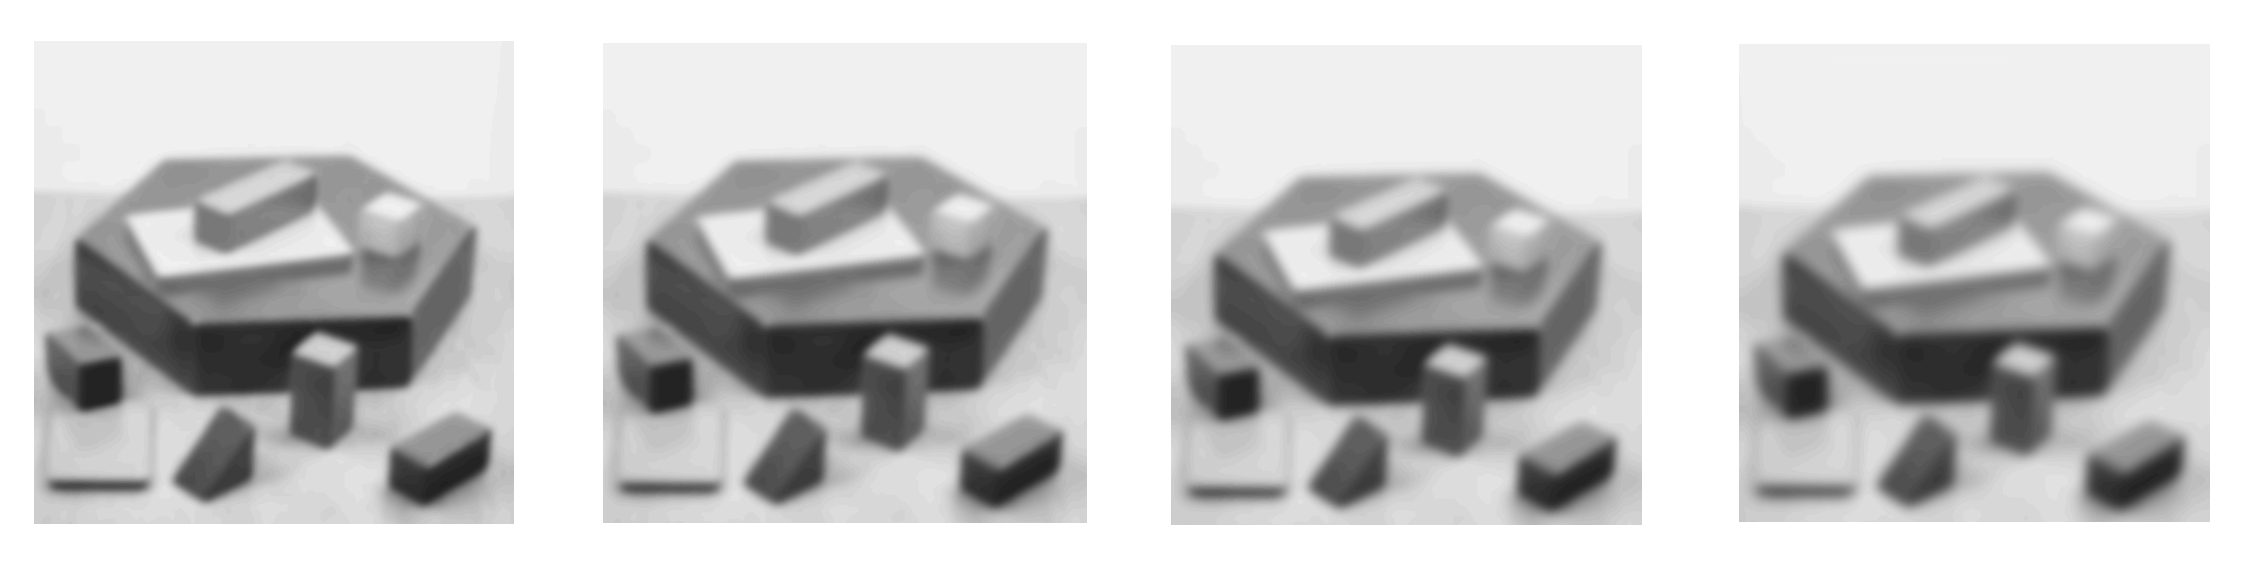
\includegraphics[width=0.8\textwidth]{Lab_3/template/figures/GaussianBlur.png}
    \caption{Resultados esperados de la generación de imágenes gaussianas}
    \label{fig:gauss_blur}
\end{figure}

\subsection*{Tarea C.1.3: Generación de diferencias de gaussianas}
\addcontentsline{toc}{subsection}{Tarea C.1.3: Generación de diferencias de gaussianas}

A partir de la lista de imágenes anteriores, se deberá generar una nueva lista con las diferencias entre las imágenes consecutivas empleando el método \texttt{subtract} \footnote{ \href{https://docs.opencv.org/3.4/d2/de8/group\_\_core\_\_array.html\#gaa0f00d98b4b5edeaeb7b8333b2de353b}{Documentación del método \texttt{cv2.subtract()} en OpenCV:} \\{https://docs.opencv.org/3.4/d2/de8/group\_\_core\_\_array.html\#gaa0f00d98b4b5edeaeb7b8333b2de353b}} de la librería \texttt{OpenCV}. La Figura \ref{fig:dog} muestra un ejemplo del resultado esperado de este apartado.

\begin{figure}[h]
    \centering
    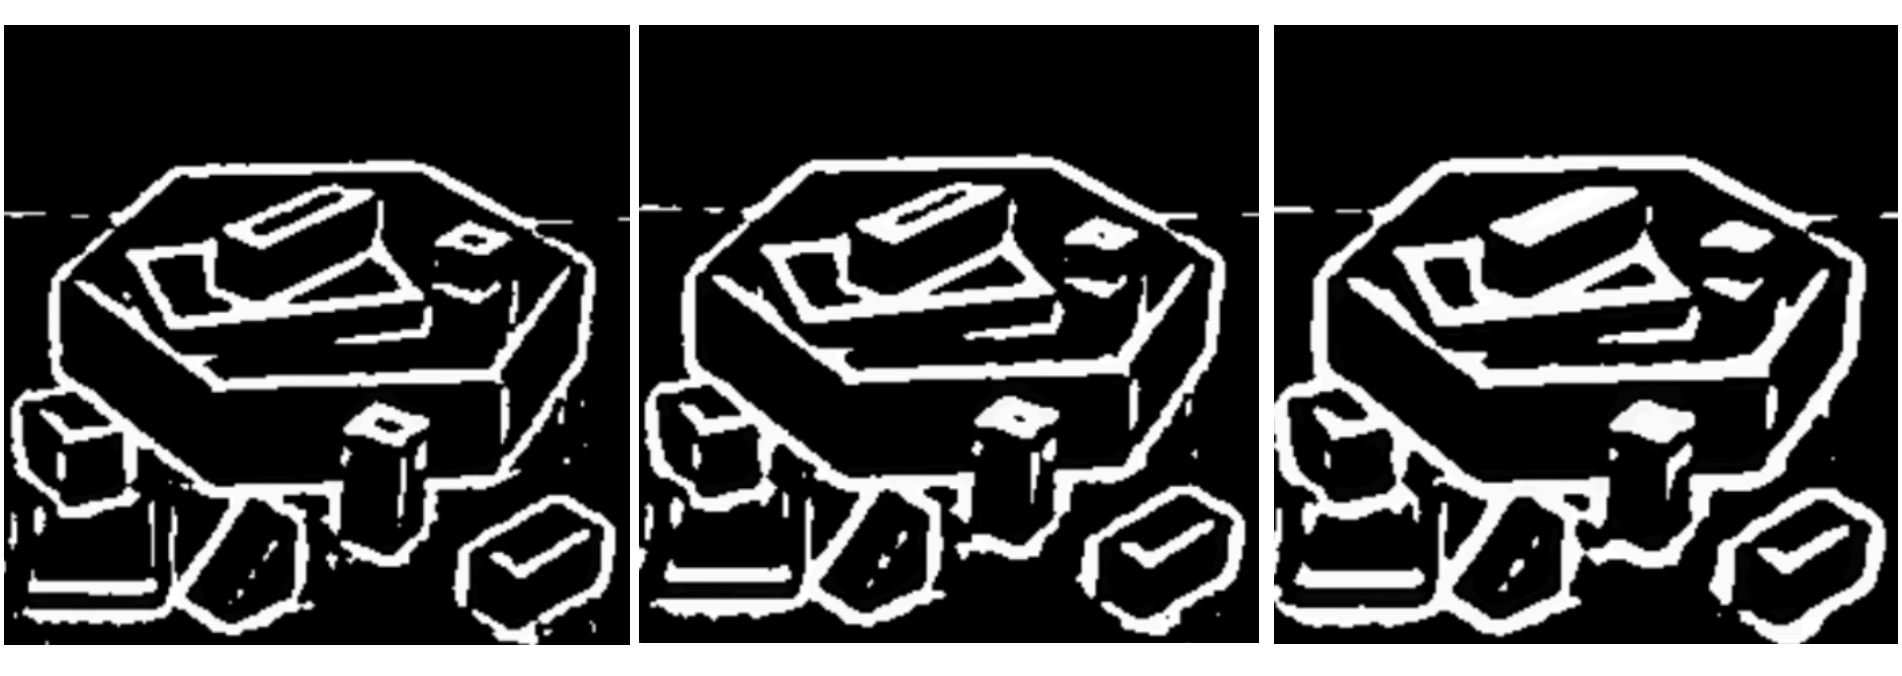
\includegraphics[width=0.8\textwidth]{Lab_3/template/figures/DoG.png}
    \caption{Resultados esperados de la generación de diferencias gaussianas}
    \label{fig:dog}
\end{figure}


\subsection*{Tarea C.1.4: Evaluación de extremos}
\addcontentsline{toc}{subsection}{Tarea C.1.4: Evaluación de extremos}

En esta tarea debe desarrollar la función \texttt{isPixelAnExtremum()} que evalua si el fixel central de una ventana de 3x3x3 es un máximo o mínimo entre sus vecinos y si es superior a un umbral mínimo en valor absoluto. La ventana está compuesta por 3 regiones de 3x3 píxeles cada una que corresponden a regiones de 3 diferencias de gaussianas consecutivas. La función debe devolver \textit{True} en caso de ser un máximo o mínimo y \textit{False} en cualquier otro caso. \textbf{Importante:} Tras el filtrado gaussiano, los píxeles pueden tener valores negativos.

\subsection*{Tarea C.1.5: Localización de puntos de interés y orientación de los mismos}
\addcontentsline{toc}{subsection}{Tarea C.1.5: Localización de puntos de interés y orientación de los mismos}

Empleando la función del apartado anterior deberá completar el desarrollo de la función \texttt{findScaleSpaceExtrema()}.

Primero tendrá que completar el bucle \texttt{for} para obtener en cada iteración 3 diferencias de gaussianas consecutivas y enumerarlas. Tras esto, iterar sobre las coordenadas de estas teniendo en cuenta que deberá mover la ventana de 3x3 a través de toda la imagen y no puede quedar ningún punto de esta ventana fuera de la misma. Complete la llamada a la función \texttt{isPixelAnExtremum()} con los argumentos pertinentes para evaluar si el pixel en las coordenadas de esa iteración es un punto extremo.

Si los píxeles son máximos o mínimos , se tiene una localización aproximada de los puntos de interés de esta imagen. La función \texttt{localizeExtremumViaQuadraticFit()} (ya proporcionada) refina esta localización teniendo en cuenta el gradiente y el hessiano; descartando los valores que no tengan el suficiente contraste. Con la localización final se obtiene la orientación del punto de interés gracias a la función \texttt{computeKeypointsWithOrientations()} (de nuevo, proporcionada). Del resultado de esta función se tiene el punto de interés definido completamente.

Se recomienda el uso de la función de borrado de duplicados (\texttt{removeDuplicateKeypoints()}, también proporcionada) ya que existen puntos de interés que se repiten en el resultado del proceso anterior. Se proporciona al alumno la función \texttt{visualizeKp()} que le permitirá visualizar los puntos de interés en la imagen original. La Figura \ref{fig:KPDet} muestra el resultado que debería obtener.

\begin{figure}[h]
    \centering
    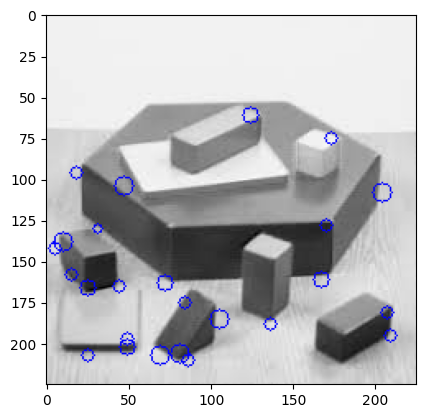
\includegraphics[width=0.4\textwidth]{Lab_3/template/figures/KeypointDetect.png}
    \caption{Resultados esperados de la detección de puntos de interés y orientación}
    \label{fig:KPDet}
\end{figure}

Una vez obtenidas las imágenes gaussianas y los puntos de interés con sus orientaciones, se pueden generar los descriptores de las regiones vecinas a estos, que son invariantes a los cambios en la iluminación y el punto de vista 3D. En esta sesión, esto se proporciona al alumno con la función \texttt{generateDescriptors()}.

\subsection*{Tarea C.1.6: \textit{Pipeline} de generación de puntos de interés y descriptores}
\addcontentsline{toc}{subsection}{Tarea C.1.6: \textit{Pipeline} de generación de puntos de interés y descriptores}

En esta tarea el alumno deberá completar la función \texttt{computeKeypointsAndDescriptors()}. Esta función recibe la imagen original, el valor inicial de \textit{sigma} y el número de diferencias de gaussianas que se desee generar. La tarea del alumno es completar la función con los métodos desarrollados en apartados anteriores para obtener el \textit{pipeline} completo de localización de puntos de interés y generación de descriptores.

\subsection*{Tarea C.1.7: Correspondencia de características entre imágenes}
\addcontentsline{toc}{subsection}{Tarea C.1.7: Correspondencia de características entre imágenes}

En esta tarea, el alumno comprobará la capacidad de sistema de localizar las mismas características en una imagen alterada para luego establecer la correspondencia entre las características de la imagen original y la de la alterada. Esto se conseguirá cargando la imagen original y la alterada en escala de grises con la librería \texttt{cv2} de \texttt{OpenCV}. Después tendrá que hacer las llamadas pertinentes al método desarrollado en el apartado anterior para obtener los puntos de interés y descriptores de ambas imágenes. 

Con estos datos, empleando la función \texttt{matchFeatures()} comprobará la capacidad de establecer la correspondencia entre los puntos de interés de ambas imágenes. La Figura \ref{fig:FMatchEnd} muestra los resultados de la correspondencia de características entre imágenes transformadas.

\begin{figure}[h]
    \centering
    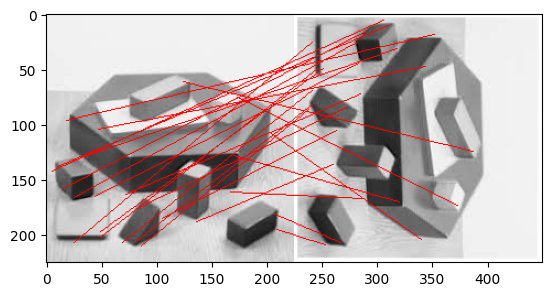
\includegraphics[width=0.8\textwidth]{Lab_3/template/figures/FeatureMatchMine.png}
    \caption{Resultados esperados de la correspondencia de características}
    \label{fig:FMatchEnd}
\end{figure}

Una vez comprendido el funcionamiento de un detector de puntos de interés y descriptores se anima al alumno a emplear el método propio de la librería \texttt{OpenCV} como se proporciona en el cuaderno.

\subsection*{Preguntas}
\addcontentsline{toc}{subsection}{Preguntas}

\vspace{5mm}
\begin{tcolorbox}[colback=gray!10, colframe=gray!30, coltitle=black, title=Pregunta C.1: Correspodencia de imágenes propias y evaluación, halign=left]
Con los métodos desarrollados para la extracción de características, haga uso del \textit{pipeline} que ha desarrollado y del método propio de\texttt{OpenCV} con sus propias imágenes. Adjunte los resultados en ambos casos y compárelos extrayendo sus propias conclusiones.
\end{tcolorbox}

\newpage
\section*{C.2: Bolsa de palabras}
\phantomsection
\addcontentsline{toc}{section}{C.2: Bolsa de palabras}

En este apartado se va a generar una bolsa de palabras a partir de un dataset de entrenamiento y se evaluará con un dataset de evaluación. Para generar la bolsa de palabras, se segirán los pasos descritos en las sesiones de teoría:

\begin{enumerate}
    \item Extracción de descriptores de puntos de interés de las imágenes del dataset.
    \item Construcción de diccionario de palabras visuales (K-Means).
    \item Para cada imagen del dataset, generar histograma de ocurrencias de palabras del diccionario.
    \item Obtener un clasificador utilizando los histogramas de las imágenes del dataset (SVM).
\end{enumerate}

De esta forma, se comenzará con la carga de las imágenes que compondrán los distintos \textit{datasets} para ser procesadas posteriormente.

\subsection*{Tarea C.2.1: Carga de \textit{datasets} de entrenamiento y validación}
\addcontentsline{toc}{subsection}{Tarea C.2.1: Carga de \textit{datasets} de entrenamiento y validación}

Como ayuda, se le proporciona una clase de Python llamada \texttt{Dataset}. Empleando el método \texttt{load()} de esta clase, cargue los \textit{datasets} de entrenamiento y validación.

\subsection*{Tarea C.2.2: Extracción de los descriptores}
\addcontentsline{toc}{subsection}{Tarea C.2.2: Extracción de los descriptores}

Una vez cargados los \textit{datasets} se puede proceder a extraer los descriptores de las imágenes que poblarán nuestra bolsa de palabras. Estos descriptores conformarán las ocurrencias de cada característica visual en la bolsa de palabras. Para ello, primero deberá cargar las imágenes del \textit{dataset} de entrenamiento con el \texttt{path} de cada una de ellas y hacerlo en escala de grises. Después, empleando los métodos necesarios de \texttt{OpenCV} que ha visto durante la sesión, genere los descriptores y guárdelos en una lista.

\subsection*{Tarea C.2.3: Creación del vocabulario}
\addcontentsline{toc}{subsection}{Tarea C.2.3: Creación del vocabulario}

Con la bolsa de palabras llena con los descriptores, se puede proceder a agrupar los mismos en las distintas palabras del vocabulario que se va a generar. Para ello, se va a ejecutar el algoritmo de clusterización de K-Means que agrupará estos descriptores. En esta tarea debe añadir los descriptores de la lista que obtuvo como resultado en la tarea anterior a la bolsa de palabras \texttt{words} que se inicializa en el código y sobre la que ejecutaremos el algoritmo. Fíjese en que se determina el número de palabras deseadas en el vocabulario final con la variable \texttt{vocabulary\_size} y que esto afectará al desempeño del clasificador más adelante.

\subsection*{Tarea C.2.4: Entrenamiento del clasificador}
\addcontentsline{toc}{subsection}{Tarea C.2.4: Entrenamiento del clasificador}

Una vez tenemos las características de las imágenes agrupadas en las palabras, se va a entrenar un clasificador que sea capaz de diferenciar entre estos grupos. Este será un modelo basado en una  \textit{Support Vector Machine}(SVM). Con este clasificador podremos recibir imágenes externas al \textit{dataset} de entrenamiento y clasificarlas en nuestro grupo de palabras.

Para entrenar el clasificador se aporta la clase \texttt{BoW} como ayuda. Añada los argumentos necesarios a los métodos especificados en la celda de código. Compruebe qué argumentos tiene que añadir accediendo al código de la clase proporcionada y analizando los métodos declarados. El modelo final se guardará en el ordenador para su uso más adelante.

\subsection*{Tarea C.2.5: Inferencia en el dataset de entrenamiento}
\addcontentsline{toc}{subsection}{Tarea C.2.5: Inferencia en el dataset de entrenamiento}

Con el modelo entrenado, es hora de ver cómo trabaja y comprobar su desempeño. En este caso la métrica empleada será la precisión y podrá observar la matriz de confusión generada para las predicciones.

Al igual que en la tarea anterior, añada los argumentos necesarios a los métodos especificados en la celda de código.

\subsection*{Tarea C.2.6: Inferencia en el dataset de validación}
\addcontentsline{toc}{subsection}{Tarea C.2.6: Inferencia en el dataset de validación}

Después de extraer los resultados con el dataset de entrenamiento, se tienen que comparar los mismos con los del dataset de validación donde se debería obtener un desempeño inferior.

Al igual que en la tarea anterior, añada los argumentos necesarios.


\subsection*{Preguntas}
\addcontentsline{toc}{subsection}{Preguntas}

\vspace{5mm}
\begin{tcolorbox}[colback=gray!10, colframe=gray!30, coltitle=black, title=Pregunta C.2.A: Cambio de SIFT por KAZE, halign=left]
Ejecute el proceso completo de nuevo cambiando el extractor de características SIFT por KAZE incluido también en la librería de \texttt{OpenCV} y en las clases de ayuda proporcionadas. Incluya el código y los resultados de inferencia en entrenamiento y validación.
\end{tcolorbox}

\vspace{5mm}
\begin{tcolorbox}[colback=gray!10, colframe=gray!30, coltitle=black, title=Pregunta C.2.B: ¿Cuantas palabras uso?, halign=left]
Como ha podido comprobar, a la hora de agrupar los descriptores y generar el vocabulario, se indica el tamaño del vocabulario y número de palabras que se desea. Itere sobre este valor y fíjese en los efectos de este sobre el desempeño final con el dataset de entrenamiento y validación. Incluya como resultados los valores empleados, la precisión obtenida y las conclusiones sobre el número adecuado de palabras a emplear.
\end{tcolorbox}
\vspace{5mm}

\begin{tcolorbox}[colback=gray!10, colframe=gray!30, coltitle=black, title=\textbf{EXTRA} - Pregunta C.2.C: En busca de los mejores parámetros, halign=left]
Al igual que ha iterado en la pregunta anterior con el número de palabras, itere con el resto de parámetros como el número de iteraciones para el K-Means, el número de iteraciones para el SVM, el extractor de caractrerísticas... Proporcione el código final con los parámetros de entrenamiento y los resultados obtenidos. El grupo que obtenga mayor precisión en validación recibirá un punto extra en la práctica.
\end{tcolorbox}


%% Prevent urls running into margins in bibliography
\setcounter{biburlnumpenalty}{7000}
\setcounter{biburllcpenalty}{7000}
\setcounter{biburlucpenalty}{7000}

%% Add bibliography
% \printbibliography[heading=bibintoc,title=References]

%% ----------------------------------------------------------------------
%%    Appendix (Letters for chapters)
%% ----------------------------------------------------------------------

%\appendix

%\chapter{Source Code Example}
%\label{chapter:title}

\emph{Adding source code to your report/thesis is supported with the package {\normalfont\texttt{listings}}. An example can be found below. Files can be added using {\normalfont\texttt{\textbackslash lstinputlisting[language=<language>]\{<filename>\}}}.}

\begin{lstlisting}[language=Python]
"""
ISA Calculator: import the function, specify the height and it will return a
list in the following format: [Temperature,Density,Pressure,Speed of Sound].
Note that there is no check to see if the maximum altitude is reached.
"""

import math
g0 = 9.80665
R = 287.0
layer1 = [0, 288.15, 101325.0]
alt = [0,11000,20000,32000,47000,51000,71000,86000]
a = [-.0065,0,.0010,.0028,0,-.0028,-.0020]

def atmosphere(h):
    for i in range(0,len(alt)-1):
        if h >= alt[i]:
            layer0 = layer1[:]
            layer1[0] = min(h,alt[i+1])
            if a[i] != 0:
                layer1[1] = layer0[1] + a[i]*(layer1[0]-layer0[0])
                layer1[2] = layer0[2] * (layer1[1]/layer0[1])**(-g0/(a[i]*R))
            else:
                layer1[2] = layer0[2]*math.exp((-g0/(R*layer1[1]))*(layer1[0]-layer0[0]))
    return [layer1[1],layer1[2]/(R*layer1[1]),layer1[2],math.sqrt(1.4*R*layer1[1])]
\end{lstlisting}

%\chapter{Task Division Example}
%\label{chapter:title}

\emph{If a task division is required, a simple template can be found below for convenience. Feel free to use, adapt or completely remove.}

\begin{table}[htb]
    \setlength\extrarowheight{4pt}
    \centering
    \caption{Distribution of the workload}
    \label{tab:taskdivision}
    \begin{tabularx}{\textwidth}{lXX}
        \toprule
        & Task & Student Name(s) \\
        \midrule
        & Summary & \\
        Chapter 1 & Introduction &  \\
        Chapter 2 &  & \\
        Chapter 3 &  & \\
        Chapter * &  & \\
        Chapter * & Conclusion &  \\
        \midrule
        & Editors & \\
        & CAD and Figures & \\
        & Document Design and Layout & \\
        \bottomrule
    \end{tabularx}
\end{table}

%\input{appendix/appendix-c} % Create file to add

\end{document}
